\documentclass[10pt,technote]{IEEEtran}


\usepackage{graphicx}
\usepackage{subcaption}
\title{Coursework 1: Face recognition }
\author{TGATH LLAG}
\begin{document}

\maketitle
\begin{abstract}
The abstract
\end{abstract}

\section{Question 1}
\subsection{Eigenfaces}
\subsubsection{Part a)}
The faces dataset consisted of 10 pictures for each of the 52 different individuals. Hence, it was decided to split the data into 7 pictures per individual for training and 3 pictures per individual for testing, resulting in a total of 364 training images. This allowed to train the PCA algorithm on all available classes and run meaningful tests on all images. Moreover, the order of pictures per individual was randomised before to remove any possible correlation between the complexity/characteristics of the pictures and their order, hinted by previous experiments. We found that with the added random component, overall, the classification accuracy improved from the initial experiments where first 7  pictures per individual were taken as the training set.

Standard PCA was performed and the eigenfaces in Figure \ref{fig:eigfaces1} were found, along with the eigenvalues in Figure \ref{fig:eigvals1}. The data was normalised by subtracting the mean face shown in Figure \ref{fig:mean_im1}. In order to identify relevant principal components, the eigenvalues of the covariance matrix with a real part lower than 0.1 were discarded (the number was chosen by inspection). 363 eigenfaces and eigenvalues remained after this thresholding operation, meaning that 363 eigenfaces were relevant to optimally reduce the dimensionality of the data. Notably, for $N$ training samples, the number of relevant eigenvalues was found to be $N - 1$. This is expected, since the largest vector subspace that can be defined with N points is R(N-1).
% How do you choose how many eigenvectors you'll actually keep ?

\begin{figure}
    \centering
    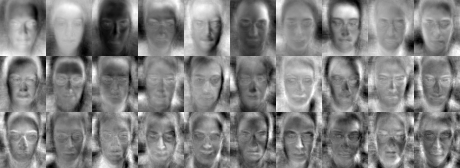
\includegraphics[width=0.4\textwidth]{../results/ex1a/eigenfaces.png}
    \caption{Eigenfaces with the 30 largest eigenvalues}
    \label{fig:eigfaces1}
\end{figure}

\begin{figure}
    \centering
    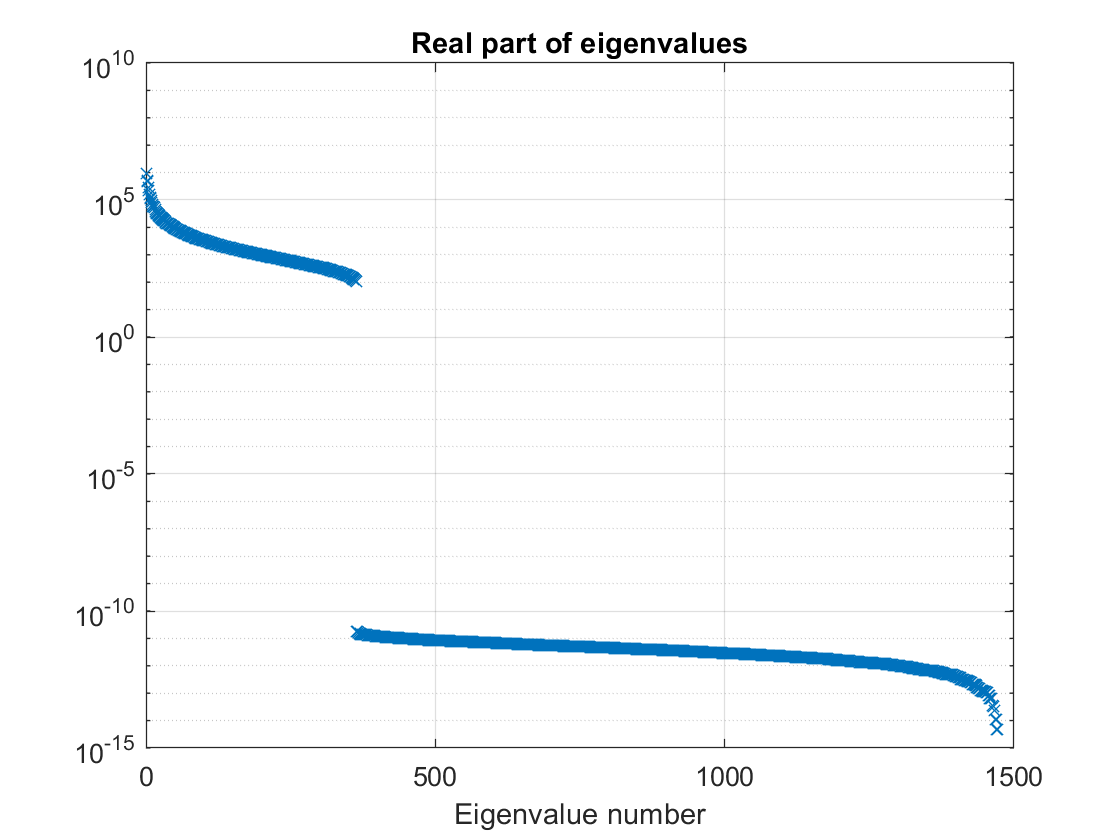
\includegraphics[width=0.4\textwidth]{../results/ex1a/eigenvalues.png}
    \caption{Real part of all PCA eigenvalues (semi-log-y axis). Negative eigenvalues were discarded but were close to 0.}
    \label{fig:eigvals1}
\end{figure}

\begin{figure}
    \centering
    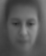
\includegraphics[width=0.1\textwidth]{../results/ex1a/mean_image.png}
    \caption{Mean image of the training dataset}
    \label{fig:mean_im1}
\end{figure}

\subsubsection{Part b)}
The low-dimensional computation returns as expected $N - 1$ eigenvalues and eigenvectors which we then compare to the original ones from Part b) in Figure \ref{fig:eig_diff1}. We can notice that there is no difference in the eigenvalue's values as well as the eigenvector's directions (by normalising them and taking their dot product). 
The low-dimensional computation proved to be 72 times faster than the standard computation, even though it involved more steps, since the dimensionality of the matrix from which the eigenvectors were computed was lower. 
% What's a con of this method ?
\begin{figure}
    \centering
    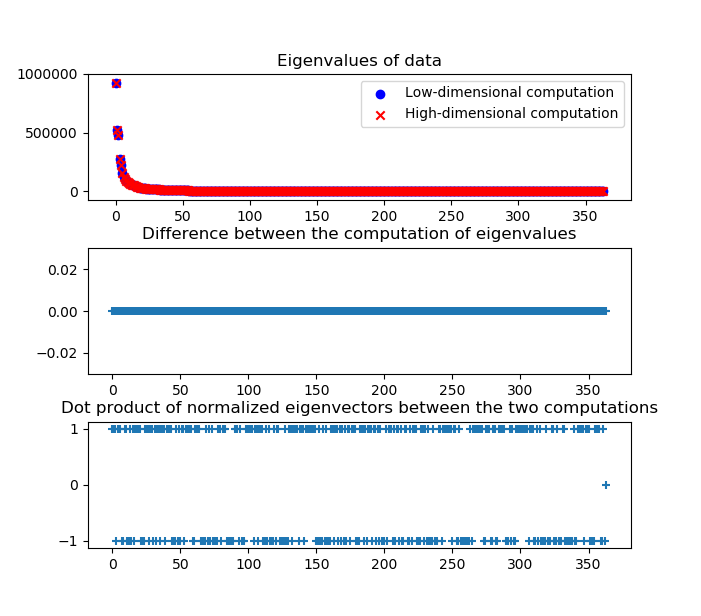
\includegraphics[width=0.5\textwidth]{../results/ex1b/DIfference_eig.png}
    \caption{Comparison of the high-dimensional and low-dimensional computations of eigenvalues and eigenvectors. Negative dot product values indicate exactly opposed vectors.}
    \label{fig:eig_diff1}
\end{figure}

\subsection{Application of eigenfaces}
\subsubsection{Part a)}
The training data was used to find the eigenfaces. The testing data was projected in the eigenspace, and it was attempted to reconstruct it by using a lower or equal amount of eigenfaces.

Quantitatively, the distortion (reconstruction error) is ever decreasing as the number of eigenvectors used for reconstruction increases, as shown in Figure \ref{fig:distortion}. However, the improvement gets slower as the number of eigenvectors increases, hinting that the full number of eigenvectors is not necessary to achieve a 'good-enough' reconstruction. As expected, when the full number of eigenvectors is used, the reconstruction is perfect (distortion of the order of $10^{-19}$)

This shows qualitatively in Figure \ref{fig:reconstr_faces}: the faces get reliably recognisable with around $M =150$ eigenvectors, whereas complex shadowing details appear only when more eigenfaces are used.
\begin{figure}
    \centering
    \begin{subfigure}[b]{0.5\textwidth}
        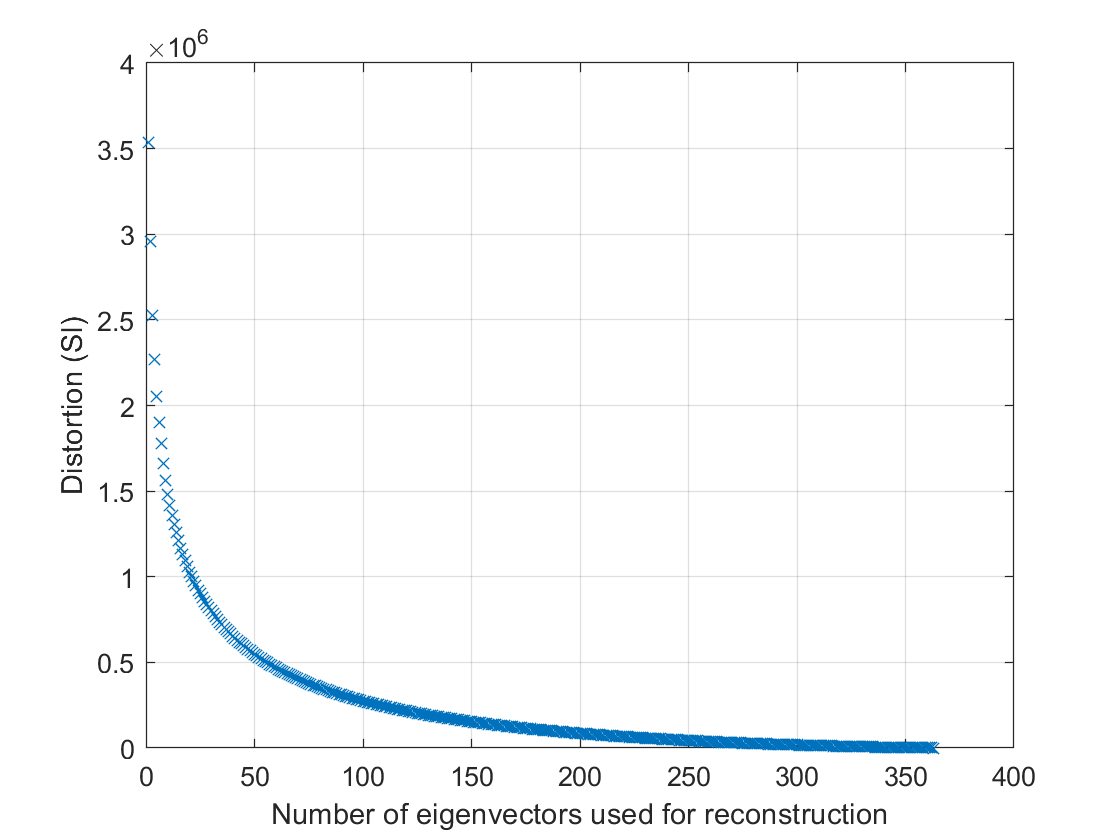
\includegraphics[width=\textwidth]{../results/ex1aa/dist_plot.png}
        \caption{Normal scale}
        
        \quad
    \end{subfigure}
    \begin{subfigure}[b]{0.5\textwidth}
        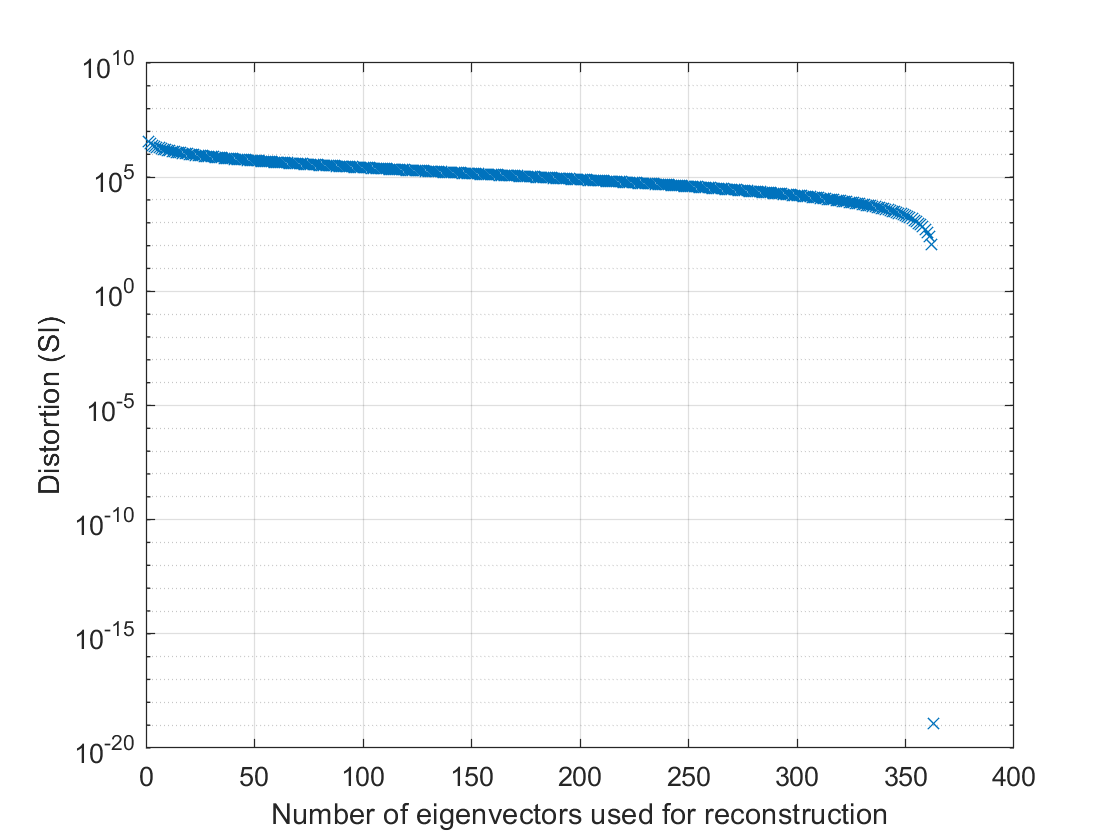
\includegraphics[width=\textwidth]{../results/ex1aa/dist_logplot.png}
        \caption{Y axis in log scale}
        
        \quad
    \end{subfigure}
    \caption{Distortion of the reconstructed images when varying the number of eigenvectors used}
    \label{fig:distortion}
\end{figure}
\begin{figure}
    \centering
    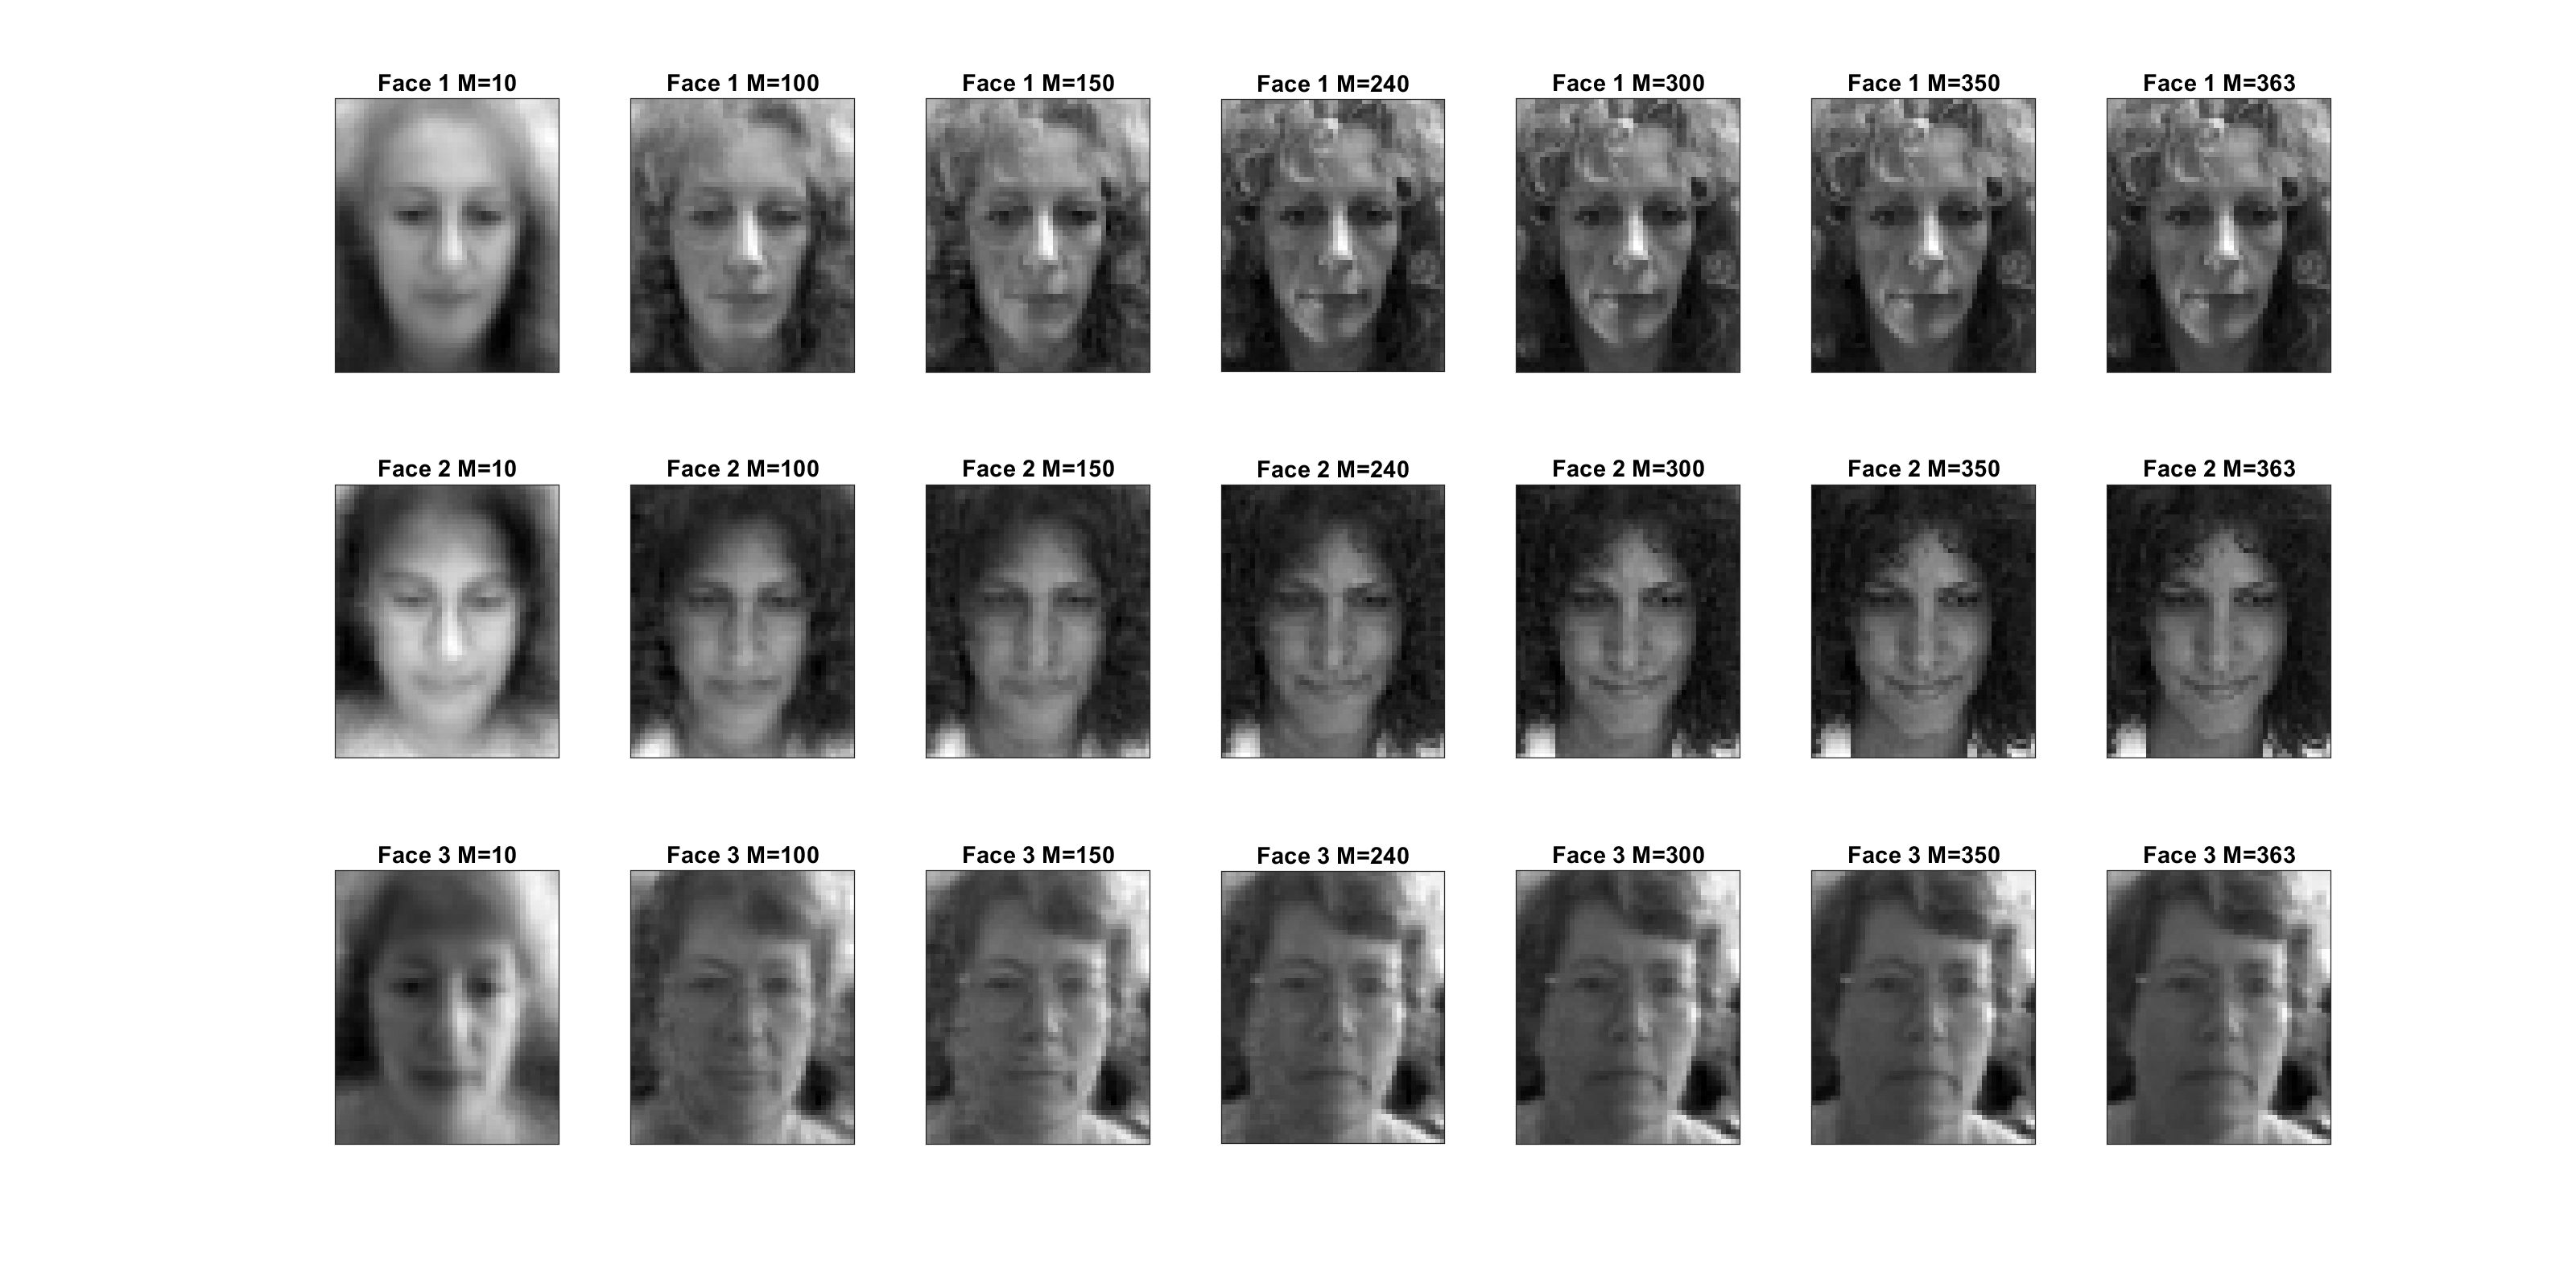
\includegraphics[width=0.5\textwidth]{../results/ex1aa/face_plots.png}
    \caption{Reconstructed faces, M indicates the number of eigenvectors used}
    \label{fig:reconstr_faces}
\end{figure}

\subsubsection{Part b)}
Table \ref{tab:NNvsRec} shows the 

\begin{table}[]
    \centering
    \begin{tabular}{c||c c}
         & NN method & Reconstruction method  \\\hline \hline\\
         Accuracy &  55 \% & 68.5 \% \\
         Duration of classification & 0.606 s & 1.05 s \\
         Peak memory usage & 104.7 MiB & 94.7 MiB
         
    \end{tabular}
    \caption{Performance comparison of face recognition using the NN method and the reconstruction method}
    \label{tab:NNvsRec}
\end{table}

\section{Question 3}
\subsection{PCA-LDA}
The data was split the same way for PCA-LDA algorithm training, with 70\% used for training and the rest for testing.

\subsection{Recognition accuracy}
Figure \ref{fig:} shows the results of the experiment where the number of retained fisher-faces ($M_{lda}$) is gradually decreased, and the dimension of the PCA subspace ($M_{pca}$) is kept as N-c. We can see that the recognition accuracy worsens as the $M_{lda}$ decreases.

In Figure \ref{fig:} we can see results of decreasing $M_{pca}$ while retaining all the fisherfaces ($c-1$).
Our results show no particular trend in decreased classification accuracy. This supports the fact that we can learn much better features when applying discriminative, supervised algorithm, making the model more successful in classifying sparse features.

\subsection{Ranks of the scatter matrices}
The scatter matrices are defined as sums of outer vector products. We confirm that the rank of the within-class-scatter matrix (Sw) is N-c. To obtain the class scatter matrix ($Si$) we remove the class-mean vector from each vector in the class, a

\subsection{PCA-LDA Ensemble}

Our model consisted of a number $T$ of sub-models made of one PCA unit and one following LDA unit. In each unit $t$, the PCA unit reduced the dimensionality of its input by applying the transform $W_{PCA}^t$, made of $M_{PCA}^t$ eigenfaces. The reduced data was then transformed by $W_{LDA}^t$, made of $M_{LDA}^t$ fisherfaces. By default, $M_{PCA}^t = N - c$ and $M_{LDA}^t = c - 1$.

\subsubsection{Bagging}

The training data was randomised and split identically to Exercise 1. However, once the training data had been obtained, it was sampled into $T$ bags, by selecting a data point uniformly from the training dataset, with replacement. This bagging technique contributed to the randomness of each unit and thus their decorrelation.
\begin{figure}
    \centering
    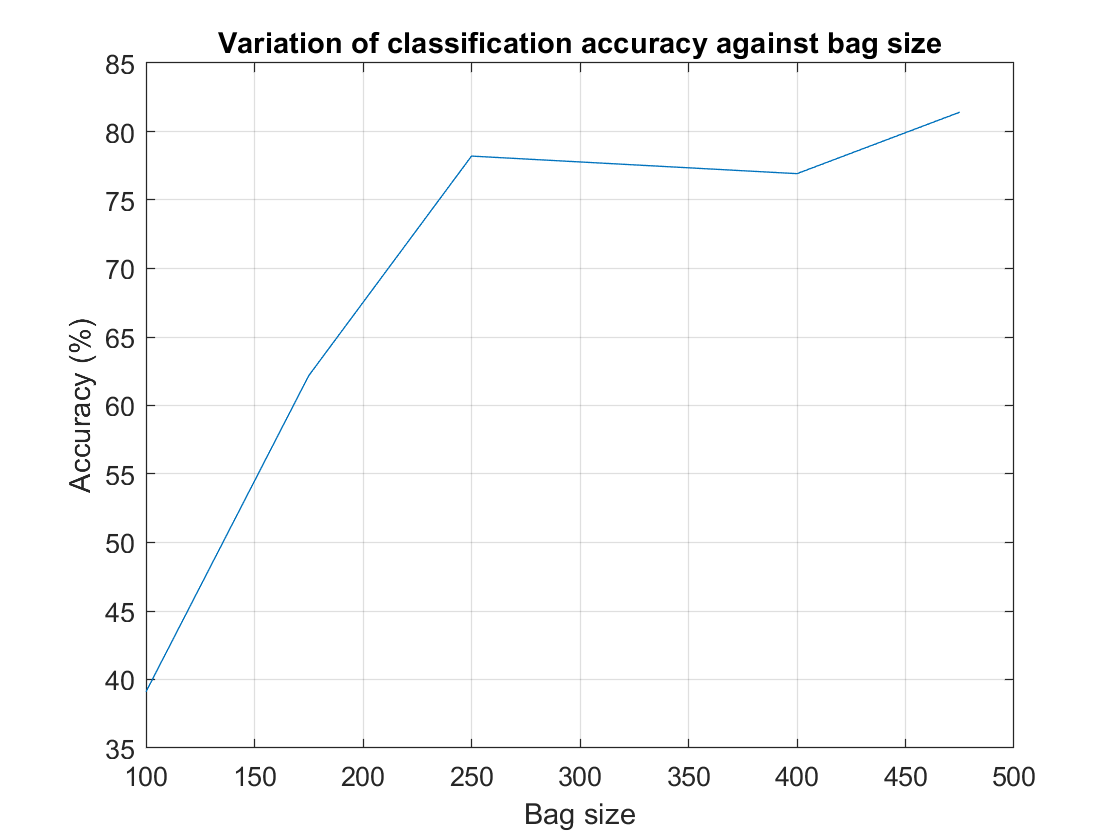
\includegraphics[width=0.7\linewidth]{../results/ex2LDAEnsemble/acc_vs_bag_size.png}
    \caption{The bag size was varied for all units simultaneously. The fusion rule was a product, T=8}
    \label{fig:acc_vs_bag}
\end{figure}
A bag size of $T = 400$ was chosen as a default value for the remaining experiments.
\subsubsection{$M_{PCA}^t$ and $M_{LDA}^t$}:
\begin{figure}
    \centering
    \begin{subfigure}[b]{0.5\textwidth}
        \includegraphics[width=\textwidth]{../results/ex2LDAEnsemble/acc_vs_M.png}
        \caption{Normal scale}
        
        \quad
    \end{subfigure}
    \begin{subfigure}[b]{0.5\textwidth}
        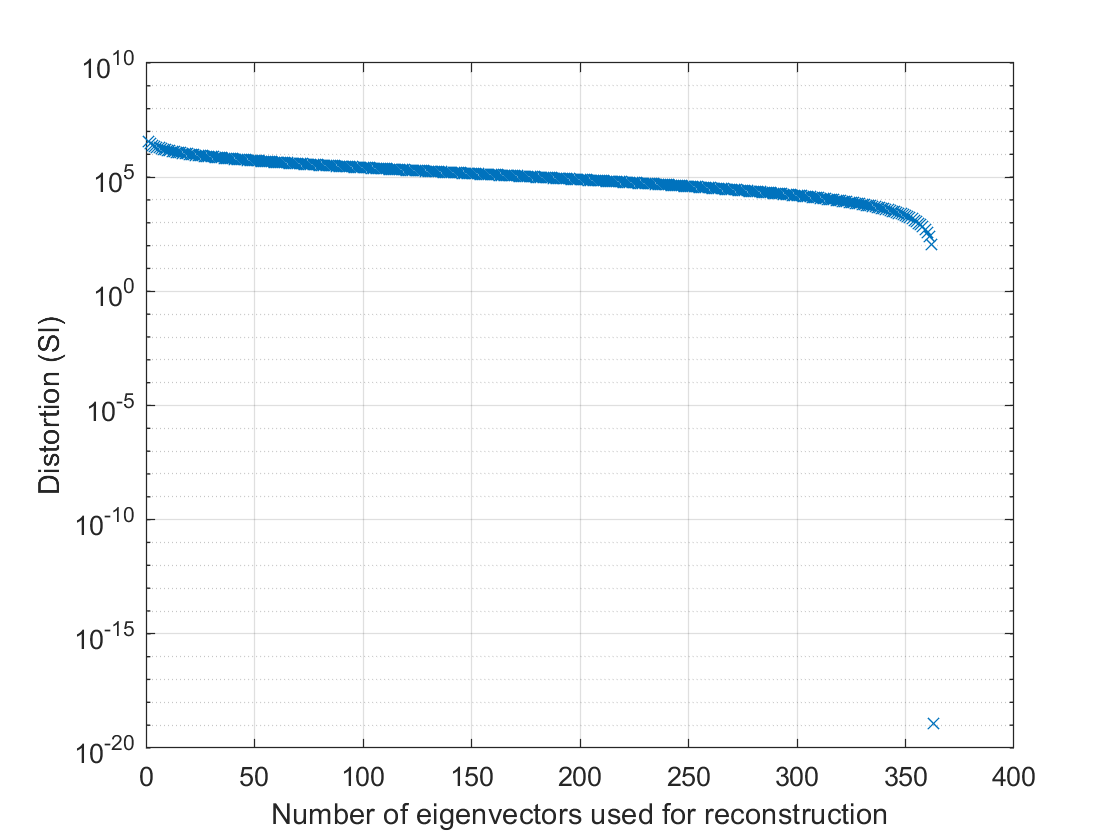
\includegraphics[width=\textwidth]{../results/ex1aa/dist_logplot.png}
        \caption{Y axis in log scale}
        
        \quad
    \end{subfigure}
    \caption{Distortion of the reconstructed images when varying the number of eigenvectors used}
    \label{fig:distortion}
\end{figure}


%\bibliography{IEEEabrv,./refs}
%\bibliographystyle{IEEEtran}

\end{document}